Das auf den folgenden Seiten vorgestellte Konzept zum spurenarmen Surfen umfasst folgende Punkte:

\begin{enumerate}
\item Die Nutzung datensammelnder Webangebote kann man vermeiden.
\item Die Annahme von Cookies und die Ausf�hrung von JavaScript wird auf vertrauensw�rdige Websites eingeschr�nkt.
\item Werbung, HTML-Wanzen und die Like-Buttons (mit denen Social Networks wie Facebook Daten sammeln) werden durch Filter blockiert.
\item Verr�terische Informationen des Browsers werden entfernt.
\item Risikoreiche und Privacy-unfreundliche Features wie PDF-Reader Plug-Ins, Browser History, Geolocation usw. werden im Browser deaktiviert.
\item HTTPS-Zertifikate werden zus�tzlich validiert, um Man-in-middle Angriffe zu erschweren.
\item Der Datenverkehr kann �ber einen Anonymisierungsdienst geleitet werden. Die verschl�sselte Kommunikation verhindert auch die Auswertung des Internetverkehrs durch mitlesende Dritte wie z.B. unsichere WLAN-Hotspots oder TK�V. (siehe \textit{Anonymymisierungsdienste nutzen})
\end{enumerate}

Mit diesen Ma�nahmen kann es vorkommen, dass Websites nicht wie erwartet funktionieren. Gute Webdesigner verzichteten auf suspekte Technologien, JavaScript wird sinnvoll eingesetzt und der Surfer auf fehlende Freigaben hingewiesen. Cookies sind meist f�r Logins n�tig und Javascript erm�glicht h�bsche Animationen oder Pr�fung von Eingaben.

\begin{center}

\includegraphics[scale=0.75]{../screenshots/cookies_required1.png}
\end{center}

Weniger gute Webseiten liefern seltsame Fehlermeldungen:

\begin{center}
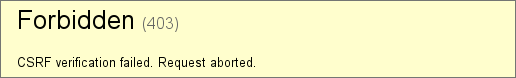
\includegraphics[scale=0.75]{../screenshots/cookies_wrong1.png}
\end{center}

Ganz schlechte Websites machen irgendwas, aber nicht was man erwartet Gelegentlich werden auch Referer oder User-Agent ausgewertet, obwohl es belanglos sein sollte, und Surfer werden nicht auf die notwendigen Freigaben hingeweisen. Hier ist man auf Probieren und Raten angewiesen. Als erstes kann man Cookies freigeben. Wenn das hilft kann man Javascript gezielt f�r einzelne Server freigeben. Ob die Deaktivierung der Schutzma�nahmen die volle Funktionalit�t aufwiegt, muss man bei Bedarf selbst entscheiden.\\

\section{Auswahl des Webbrowsers}
Firefox ist der Webbrowser der Mozilla Foundation. Er ist kostenfrei nutzbar und steht auf der Website des Projektes \footnote{ \href{http://www.mozilla-europe.org/de/firefox}{http://www.mozilla-europe.org/de/firefox}} f�r fast alle Betriebssystem zum Download bereit. Linux-Distributionen enthalten den Browser in der Regel.\\

Debian GNU/Linux enth�lt eine branded version des Browsers unter dem Namen \textit{Iceweasel}, allerding oft in einer veralteten Version. Das Mozilla Debian Team stellt eine aktuelle Version in einem extra Repository \footnote{ \href{http://mozilla.debian.net}{http://mozilla.debian.net}} bereit.\\

Firefox kann durch viele von der Community entwickelte Add-ons und Anpassungen in der Konfiguration zu einem sicheren und privacy-freundlichen Browser aufgewertet werden. Ich beschr�nke mich im folgenden auf diesen einen Browser. Das ist schon sehr umfangreich, wenn man es gut machen will.

\subsubsection*{JonDoFox}
Der JonDoFox\footnote{ \href{https://www.anonym-surfen.de/jondofox.html}{https://www.anonym-surfen.de/jondofox.html}} ist ein Browser-Profil f�r Firefox, dass alle Einstellungen umsetzt, die auf den folgenden Seiten beschrieben werden. Nach der Installation von Mozilla Firefox ist das JonDoFox-Profil zus�tzlich zu installieren - fertig. Zuk�nftig fragt Firefox bei jedem Start, welches Profil genutzt werden soll. JonDoFox ist f�r anonymes Surfen mit JonDonym entwickelt worden, kann aber auch ohne Anonymisierungsdienst verwendet werden, indem man in der Statuszeile unten rechts auf \textit{Kein Proxy} oder \textit{Benutzerdefiniert} umschaltet.

\begin{center}
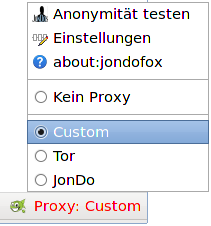
\includegraphics[scale=0.75]{../screenshots/jondofox-proxy-ohne.png}
\end{center}

Wenn man den Proxy \textit{Benutzerdefiniert} w�hlt, kann die User-Agent Kennung modifiziert werden. Das ist vor allem f�r Nutzer seltener Betriebssysteme sinnvoll, um sich in der Masse der Windows-Nutzer zu verstecken. In den Einstellungen des JonDoFox kann man f�r Benutzerdefinierte Proxys den \textit{Firefox 17.0 f�r Windows} (JonDo) oder \textit{Firefox 10.0 f�r Windows} (Tor) als Fake zu nutzen. Mit dieser kleinen Anpassung erh�lt man einen optimal konfigurierten Browser. Das folgende Kapitel kann man trotzdem lesen oder �berfliegen, um die damit verbundenen Einschr�nkungen besser zu verstehen.\\

\begin{figure}[htb]
\begin{center}
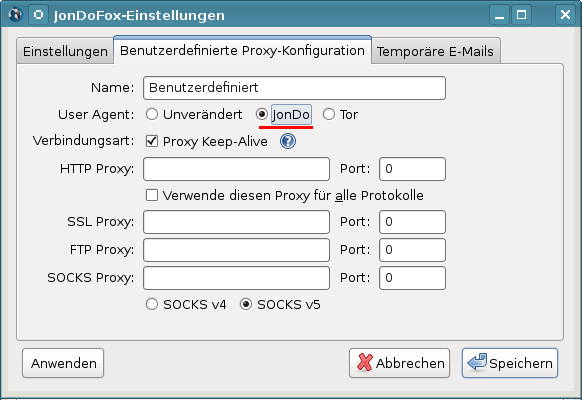
\includegraphics[scale=0.7]{../screenshots/jondofox-ua-ohne.png}
\caption{User-Agent Kennung konfigurieren}
\label{abb:jondofox-ua}
\end{center}
\end{figure}

Eine kurze Einf�hrung in den Umgang mit JonDoFox gibt es im Kapitel Anonymisierungsdienste.

\subsubsection*{JoDoBrowser}
Der JonDoBrowser\footnote{ \href{https://www.anonym-surfen.de/jondobrowser.html}{https://www.anonym-surfen.de/jondobrowser.html}} ist nicht nur sicher konfiguriert sondern enth�lt auch Modifikationen im Source Code von Mozilla Firefox, um eine h�here Anonymit�t zu bieten. Die aktuelle Beta Version arbeitet stabil und kann meiner Meinung nach f�r die t�gliche Arbeit eingesetzt werden.\\

Standardm��ig ist die Proxy-Umschaltung im JonDoBrowser deaktiviert. Das erweiterte Men� muss erst in den Einstellungen des JonDoFox-XPI (siehe Bild \ref{abb:proxyfreigeben}) aktiviert werden. Dann kann man wie beim JonDoFox auf \textit{``Kein Proxy``} umschalten und ohne Anonymisierungsdienst spurenarm surfen.

\begin{figure}[htb]
\begin{center}
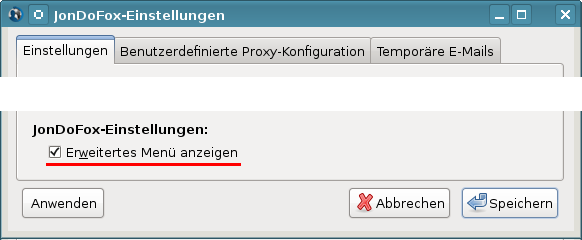
\includegraphics[scale=0.7]{../screenshots/jondobrowser-proxy-aktivieren.png}
\caption{Proxy-Umschaltung im JonDoBrowser freigeben}
\label{abb:proxyfreigeben}
\end{center}
\end{figure}